\documentclass[a4paper, 10pt]{article}
\usepackage[siunitx]{circuitikz}
\usepackage[margin=1in]{geometry}
\usepackage{subfiles}

\usetikzlibrary{intersections}

\begin{document}
\tikzset{blockdef-above/.style={%
	{Straight Barb[harpoon, right, length=-0.2cm]}-{Straight Barb[harpoon, left, length=-0.2cm]},
	black,
	}}

\tikzset{blockdef-below/.style={%
	{Straight Barb[harpoon, reversed, right, length=0.2cm]}-{Straight Barb[harpoon, reversed, left, length=0.2cm]},
	black,
	}}

\def\gateTransistor{$BC547$}
\def\baseResistor{\SI{220}{k\ohm}}
\def\outResistor{\SI{47}{k\ohm}}
\def\ledResistor{\SI{18}{k\ohm}}
\def\vccPotential{$V_{CC}=\SI{5}{V}$}

\clearpage

\section{Logic Gates}

\subsection{AND Gate}

\begin{figure}[!ht]
	\centering
    \includegraphics{tikzpics/epictlvlandgate.pdf}
	\caption{\textbf{AND} Gate}
\end{figure}

\subsection{OR Gate}

\begin{figure}[!hb]
	\centering
    \includegraphics{tikzpics/epictlvlorgate.pdf}
	\caption{\textbf{OR} Gate}
\end{figure}

\subsection{XOR Gate}

\begin{figure}[!hp]
	\centering
    \includegraphics{tikzpics/epictlvlxorgate.pdf}
	\caption{\textbf{XOR} Gate}
\end{figure}

\clearpage

\section{Adders}

\subsection{Half Adder}

\begin{figure}[!ht]
	\centering
    \includegraphics{tikzpics/epicglvlhalfadder.pdf}
	\caption{Half Adder}
\end{figure}

\vspace{0.2\textheight}

\subsection{Full Adder}

\begin{figure}[!hb]
	\centering
    \includegraphics{tikzpics/epicglvlfulladder.pdf}
	\caption{Full Adder}
\end{figure}

\clearpage

\subsection{Full Adder from Raw \textbf{Transistors}}

\begin{figure}[!h]
	\centering
	\resizebox{\textwidth}{!}{
    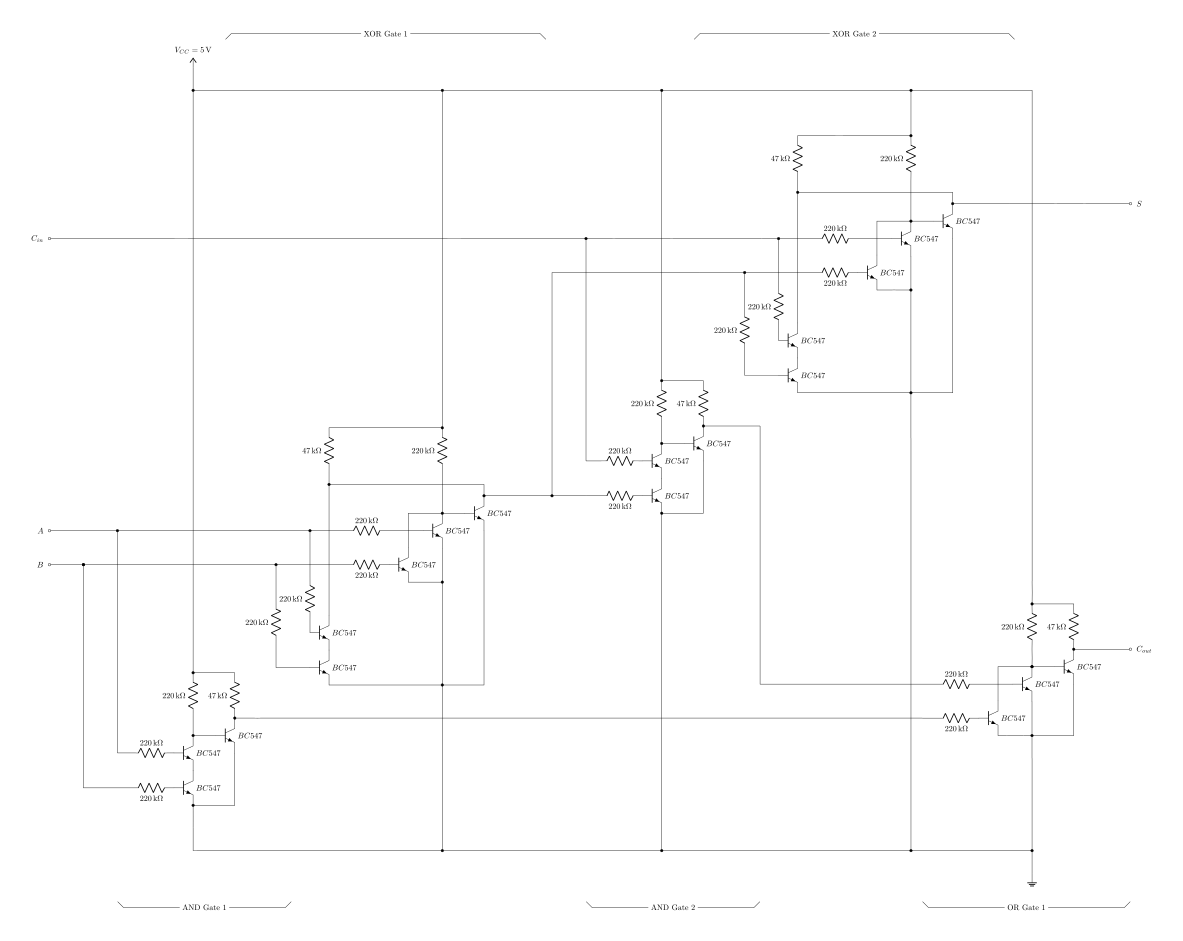
\includegraphics{tikzpics/epictlvlfulladder.pdf}
	}
	\caption{Full Adder from Raw \textbf{Transistors}}
\end{figure}

\clearpage

\section{Control Module}

\subsection{Control Module for 4 bit Ripple Adder}

\begin{figure}[!h]
	\centering
	\resizebox{!}{0.8\textheight}{
		\begin{circuitikz}[american, rotate=-90, transform shape]

			\draw

			% SA4

			(0,0)
			node (SA4) [spdt, anchor=in] {}

			(SA4.in) to[short, -*] ++(-0.5,0)
			coordinate (SA4-br)
			to[R, l=\ledResistor] ++(0,-2)
			to[leDo] ++(0,-2)
			coordinate (SA4-lend)

			(SA4.out 1) -- ++(0.5,0)
			coordinate (SA4-outbr)

			% SA3

			(SA4.in-|SA4.out 1) ++(5,1)
			node (SA3) [spdt, anchor=in] {}

			(SA3.in) to[short, -*] ++(-0.5,0)
			coordinate (SA3-br)
			to[R, l=\ledResistor] ++(0,-2)
			to[leDo] ++(0,-2)
			coordinate (SA3-lend)

			(SA3.out 1) -- ++(0.5,0)
			coordinate (SA3-outbr)

			% SA2

			(SA3.in-|SA3.out 1) ++(5,1)
			node (SA2) [spdt, anchor=in] {}

			(SA2.in) to[short, -*] ++(-0.5,0)
			coordinate (SA2-br)
			to[R, l=\ledResistor] ++(0,-2)
			to[leDo] ++(0,-2)
			coordinate (SA2-lend)

			(SA2.out 1) -- ++(0.5,0)
			coordinate (SA2-outbr)

			% SA1

			(SA2.in-|SA2.out 1) ++(5,1)
			node (SA1) [spdt, anchor=in] {}

			(SA1.in) to[short, -*] ++(-0.5,0)
			coordinate (SA1-br)
			to[R, l=\ledResistor] ++(0,-2)
			to[leDo] ++(0,-2)
			coordinate (SA1-lend)

			(SA1.out 1) -- ++(0.5,0)
			coordinate (SA1-outbr)

			% SB4

			(SA4.in-|SA4.out 1) ++(1.9,0) % my OCD :(
			coordinate (tmp)
			(tmp|-SA4-lend) ++(0,-4)

			node (SB4) [spdt, anchor=in] {}

			(SB4.in) to[short, -*] ++(-0.5,0)
			coordinate (SB4-br)
			to[R, l=\ledResistor] ++(0,-2)
			to[leDo] ++(0,-2)
			coordinate (SB4-lend)

			(SB4.out 1) -- ++(0.5,0)
			coordinate (SB4-outbr)

			% SB3

			(SB4.in-|SB4.out 1) ++(5,1)
			node (SB3) [spdt, anchor=in] {}

			(SB3.in) to[short, -*] ++(-0.5,0)
			coordinate (SB3-br)
			to[R, l=\ledResistor] ++(0,-2)
			to[leDo] ++(0,-2)
			coordinate (SB3-lend)

			(SB3.out 1) -- ++(0.5,0)
			coordinate (SB3-outbr)

			% SB2

			(SB3.in-|SB3.out 1) ++(5,1)
			node (SB2) [spdt, anchor=in] {}

			(SB2.in) to[short, -*] ++(-0.5,0)
			coordinate (SB2-br)
			to[R, l=\ledResistor] ++(0,-2)
			to[leDo] ++(0,-2)
			coordinate (SB2-lend)

			(SB2.out 1) -- ++(0.5,0)
			coordinate (SB2-outbr)

			% SB1

			(SB2.in-|SB2.out 1) ++(5,1)
			node (SB1) [spdt, anchor=in] {}

			(SB1.in) to[short, -*] ++(-0.5,0)
			coordinate (SB1-br)
			to[R, l=\ledResistor] ++(0,-2)
			to[leDo] ++(0,-2)
			coordinate (SB1-lend)

			(SB1.out 1) -- ++(0.5,0)
			coordinate (SB1-outbr)


			% A input

			(SA4-br)
			to[short, -o] ++(-3,0)
			coordinate (A4)
			node () [left=4pt] {$A_{4}$}

			(SA3-br)
			to[short, -o] (SA3-br-|A4)
			coordinate (A3)
			node () [left=4pt] {$A_{3}$}

			(SA2-br)
			to[short, -o] (SA2-br-|A4)
			coordinate (A2)
			node () [left=4pt] {$A_{2}$}

			(SA1-br)
			to[short, -o] (SA1-br-|A4)
			coordinate (A1)
			node () [left=4pt] {$A_{1}$}


			% B input

			(SB4-br)
			to[short, -o] (SB4-br-|A4)
			coordinate (B4)
			node () [left=4pt] {$B_{4}$}

			(SB3-br)
			to[short, -o] (SB3-br-|A4)
			coordinate (B3)
			node () [left=4pt] {$B_{3}$}

			(SB2-br)
			to[short, -o] (SB2-br-|A4)
			coordinate (B2)
			node () [left=4pt] {$B_{2}$}

			(SB1-br)
			to[short, -o] (SB1-br-|A4)
			coordinate (B1)
			node () [left=4pt] {$B_{1}$}


			% Output

			(SB1-outbr|-SB4-lend) ++(3,2)
			node (nb5) [npn, xscale=-1, anchor=E] {
				\scalebox{-1}[1]{\gateTransistor}}
			(nb5.C)
			to[leDo, mirror, invert] ++(0,2)
			to[R, l=\ledResistor] ++(0,2)
			coordinate (nb5-lend)
			(nb5.B)
			to[R, l_=\baseResistor] ++(2,0)
			coordinate (nb5-bend)

			(nb5.E) ++(3,1)
			node (nb4) [npn, xscale=-1, anchor=E] {
				\scalebox{-1}[1]{\gateTransistor}}
			(nb4.C)
			to[leDo, mirror, invert] ++(0,2)
			to[R, l=\ledResistor] ++(0,2)
			coordinate (nb4-lend)
			(nb4.B)
			to[R, l_=\baseResistor] ++(2,0)
			coordinate (nb4-bend)

			(nb4.E) ++(3,1)
			node (nb3) [npn, xscale=-1, anchor=E] {
				\scalebox{-1}[1]{\gateTransistor}}
			(nb3.C)
			to[leDo, mirror, invert] ++(0,2)
			to[R, l=\ledResistor] ++(0,2)
			coordinate (nb3-lend)
			(nb3.B)
			to[R, l_=\baseResistor] ++(2,0)
			coordinate (nb3-bend)

			(nb3.E) ++(3,1)
			node (nb2) [npn, xscale=-1, anchor=E] {
				\scalebox{-1}[1]{\gateTransistor}}
			(nb2.C)
			to[leDo, mirror, invert] ++(0,2)
			to[R, l=\ledResistor] ++(0,2)
			coordinate (nb2-lend)
			(nb2.B)
			to[R, l_=\baseResistor] ++(2,0)
			coordinate (nb2-bend)

			(nb2.E) ++(3,1)
			node (nb1) [npn, xscale=-1, anchor=E] {
				\scalebox{-1}[1]{\gateTransistor}}
			(nb1.C)
			to[leDo, mirror, invert] ++(0,2)
			to[R, l=\ledResistor] ++(0,2)
			coordinate (nb1-lend)
			(nb1.B)
			to[R, l_=\baseResistor] ++(2,0)
			coordinate (nb1-bend)

			% O output

			(nb1-bend)
			to[short, -o] ++(2,0)
			coordinate (O1)
			node () [right=4pt] {$O_{1}$}

			(nb2-bend)
			to[short, -o] (nb2-bend-|O1)
			coordinate (O2)
			node () [right=4pt] {$O_{2}$}

			(nb3-bend)
			to[short, -o] (nb3-bend-|O1)
			coordinate (O3)
			node () [right=4pt] {$O_{3}$}

			(nb4-bend)
			to[short, -o] (nb4-bend-|O1)
			coordinate (O2)
			node () [right=4pt] {$O_{4}$}

			(nb5-bend)
			to[short, -o] (nb5-bend-|O1)
			coordinate (Cfinal)
			node () [right=4pt] {$C_{final}$}

			% Carry initial

			(SA4-lend|-SB4-lend)
			to[short, *-o] (A1|-SB4-lend)
			coordinate (Cinitial)
			node [left=4pt] {$C_{initial}$}

			% Supply out

			(SA1-outbr|-SA1.out 2) ++(0,-1)
			coordinate (tmp)
			to[short, *-o] (O1|-tmp)
			coordinate (Gout)
			node [right=4pt] {$G_{out}$}

			(Gout) ++(0,1)
			coordinate (Vout)
			to[short, o-*] (SB1-outbr|-Vout)
			(Vout)
			node [right=4pt] {$V_{out}$}

			% ground

			(SB4-lend) to[short, -*] ++(0,-1)
			coordinate (Gbr)

			(SB4.out 2) -- (SB4-outbr|-SB4.out 2)
			to[short, -*] (SB4-outbr|-Gbr)
			(SB3.out 2) -- (SB3-outbr|-SB3.out 2)
			to[short, -*] (SB3-outbr|-Gbr)
			(SB2.out 2) -- (SB2-outbr|-SB2.out 2)
			to[short, -*] (SB2-outbr|-Gbr)
			(SB1.out 2) -- (SB1-outbr|-SB1.out 2)
			to[short, -*] (SB1-outbr|-Gbr)

			(SA4.out 2) -- (SA4-outbr|-SA4.out 2)
			to[short, -*] (SA4-outbr|-Gbr)
			(SA3.out 2) -- (SA3-outbr|-SA3.out 2)
			to[short, -*] (SA3-outbr|-Gbr)
			(SA2.out 2) -- (SA2-outbr|-SA2.out 2)
			to[short, -*] (SA2-outbr|-Gbr)
			(SA1.out 2) -- (SA1-outbr|-SA1.out 2)
			to[short, -*] (SA1-outbr|-Gbr)

			(SA4-lend) to[short, -] (SA4-lend|-Gbr)
			(SA3-lend) to[short, -*] (SA3-lend|-Gbr)
			(SA2-lend) to[short, -*] (SA2-lend|-Gbr)
			(SA1-lend) to[short, -*] (SA1-lend|-Gbr)

			(SB3-lend) to[short, -*] (SB3-lend|-Gbr)
			(SB2-lend) to[short, -*] (SB2-lend|-Gbr)
			(SB1-lend) to[short, -*] (SB1-lend|-Gbr)

			(nb5.E) to[short, -*] (nb5.E|-Gbr)
			(nb4.E) to[short, -*] (nb4.E|-Gbr)
			(nb3.E) to[short, -*] (nb3.E|-Gbr)
			(nb2.E) to[short, -*] (nb2.E|-Gbr)
			(nb1.E) to[short, -] (nb1.E|-Gbr)

			(SA4-lend|-Gbr)
			to[short, -*] (nb1.E|-Gbr)
			-- ++(0,-1.5)
			coordinate (G)
			node [ground] {}

			% vcc

			(SA1-outbr) to[short, -*] ++(0,1.5)
			coordinate (Vbr)

			(SA4-outbr) to[short, -] (SA4-outbr|-Vbr)
			(SA3-outbr) to[short, -*] (SA3-outbr|-Vbr)
			(SA2-outbr) to[short, -*] (SA2-outbr|-Vbr)
			(SA1-outbr) to[short, -*] (SA1-outbr|-Vbr)

			(SB4-outbr) to[short, -*] (SB4-outbr|-Vbr)
			(SB3-outbr) to[short, -*] (SB3-outbr|-Vbr)
			(SB2-outbr) to[short, -*] (SB2-outbr|-Vbr)
			(SB1-outbr) to[short, -*] (SB1-outbr|-Vbr)


			(nb5-lend) to[short, -*] (nb5-lend|-Vbr)
			(nb4-lend) to[short, -*] (nb4-lend|-Vbr)
			(nb3-lend) to[short, -*] (nb3-lend|-Vbr)
			(nb2-lend) to[short, -*] (nb2-lend|-Vbr)
			(nb1-lend) to[short, -] (nb1-lend|-Vbr)

			(nb1-lend|-Vbr)
			to[short, -*] (SA4-outbr|-Vbr)
			-- ++(0,1.5)
			coordinate (V)
			node [vcc] {\vccPotential}

			;

		\end{circuitikz}
		}
		\caption{Control Module for \textbf{4 bit Ripple Adder}}
	\end{figure}


\clearpage

\subsection{Control Module for Full Adder}

\begin{figure}[!h]
	\centering
	\resizebox{\textwidth}{!}{
		\begin{circuitikz}[american]

		\draw (0,0)
		node (S1) [spdt] {}

		(S1.in) to[short, -*] ++(-0.5,0)
		coordinate (S1br)
		to[short, -o] ++(-2,0)
		coordinate (A)
		node [left=4pt] {$A$}

		(S1br) -- ++(0,-0.5)
		to[R, l=\ledResistor] ++(0,-2)
		to[leDo] ++(0,-2)
		-- ++(0,-0.5)
		coordinate (Gbr)

		(S1.out 2) -- ++(0.5,0)
		coordinate (S1outbr)
		to[short, -*] (S1outbr|-Gbr)

		(S1.out 1) -- (S1.out 1-|S1outbr)
		to[short, -*] ++($(S1.out 2)-(S1.out 2|-Gbr)$)
		coordinate (Vbr)

		(S1.out 1) ++(4.5,1)
		node (S2) [spdt, anchor=out 1] {}
		(S2.out 1) -- ++(0.5,0)
		coordinate (S2outbr)

		to[short, -*] (S2outbr|-Vbr)
		(S2.out 2) -- (S2outbr|-S2.out 2)
		to[short, -*] (S2outbr|-Gbr)

		(S2.in) to[short, -*] ++(-0.5,0)
		coordinate (S2br)
		to[short, -o] (S2br-|A)
		coordinate (B)
		node [left=4pt] {$B$}

		(S2br) to[R, l=\ledResistor] ++(0,-2)
		to[leDo] ++(0,-2)
		to[short, -*] (S2br|-Gbr)

		(S2.out 1) ++(4.5,1)
		node (S3) [spdt, anchor=out 1] {}
		(S3.out 1) -- ++(0.5,0)
		coordinate (S3outbr)

		to[short, -*] (S3outbr|-Vbr)
		(S3.out 2) -- (S3outbr|-S3.out 2)
		to[short, -*] (S3outbr|-Gbr)

		(S3.in) to[short, -*] ++(-0.5,0)
		coordinate (S3br)
		to[short, -o] (S3br-|A)
		coordinate (Cin)
		node [left=4pt] {$C_{in}$}

		(S3br) to[R, l=\ledResistor] ++(0,-2)
		to[leDo] ++(0,-2)
		to[short, -*] (S3br|-Gbr)

		(S1.in-|S3.in) ++(4,0)
		node (nb1) [npn, xscale=-1, anchor=C] {
			\scalebox{-1}[1]{\gateTransistor}}

		(nb1.C) -- ++(0,-0.5)
		to[leDo, invert, mirror] ++(0,2)
		to[R, l=\ledResistor] ++(0,2)
		to[short, -*] (nb1.C|-Vbr)

		(nb1.E) to[short, -*] (nb1.E|-Gbr)

		(nb1.B) -- ++(2.25,0)
		to[R, l=\baseResistor] ++(2,0)
		to[short, -o] ++(0.5,0)
		coordinate (S)
		node [right=4pt] {$S$}

		(nb1.C) ++(2.25,1)
		node (nb2) [npn, xscale=-1, anchor=C] {
			\scalebox{-1}[1]{\gateTransistor}}

		(nb2.C) -- ++(0,-0.5)
		to[leDo, invert, mirror] ++(0,2)
		to[R, l=\ledResistor] ++(0,2)
		-- (nb2.C|-Vbr)

		(nb2.E) to[short, -*] (nb2.E|-Gbr)

		(nb2.B) to[R, l=\baseResistor] ++(2,0)
		to[short, -o] (nb2.B-|S)
		coordinate (Cout)
		node [right=4pt] {$C_{out}$}

		(Cin) ++($(Cin)-(B)$)
		coordinate (Vout)
		node [left=4pt] {$V_{out}$}
		to[short, o-*] (Vout-|S3outbr)

		(S) ++($(S)-(Cout)$)
		coordinate (Gout)
		node [right=4pt] {$G_{out}$}
		to[short, o-*] (Gout-|S3outbr)

		(nb2.C|-Vbr) -- (S1outbr|-Vbr)
		-- ++(0,1.5)
		coordinate (V)
		node [vcc] {\vccPotential}

		(S1br|-Gbr) -- (nb2.E|-Gbr)
		-- ++(0,-1.5)
		coordinate (G)
		node [ground] {}

		;

	\end{circuitikz}
	}
	\caption{Control Module for \textbf{Full Adder}}
\end{figure}

\end{document}
